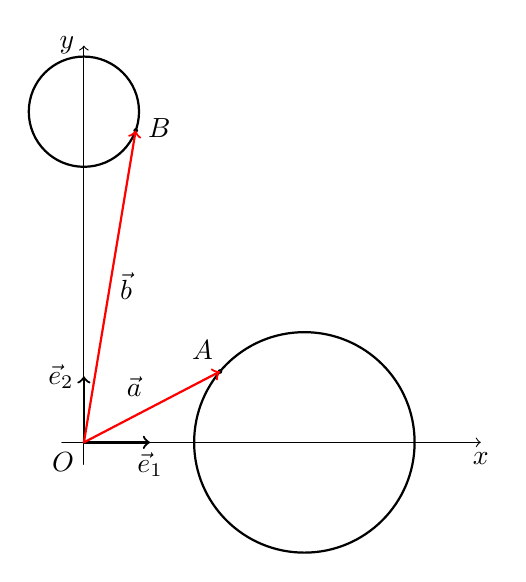
\begin{tikzpicture}[line cap=round,line join=round,scale=0.7]
\usetikzlibrary{calc}

% ---- axes (with dashed inner guides like the picture) ----
\draw[->] (-0.4,0) -- (7.2,0) node[below] {$x$};
\draw[->] (0,-0.4) -- (0,7.2) node[left] {$y$};
\node[below left] at (0,0) {$O$};

% unit vectors e1,e2
\draw[->,thick] (0,0) -- (1.2,0) node[below] {$\vec e_1$};
\draw[->,thick] (0,0) -- (0,1.2) node[left] {$\vec e_2$};

% ---- circles: C1 centered at (4,0) radius 2; C2 centered at (0,6) radius 1 ----
\draw[thick] (4,0) circle (2);
\draw[thick] (0,6) circle (1);


% ---- points A on C1 and B on C2 (choose a representative placement) ----
\coordinate (A) at ($(4,0)+(140:2)$);
\coordinate (B) at ($(0,6)+(-20:1)$);

\fill (A) circle (1.2pt);
\node[above left] at ($(A)+(0.05,0.05)$) {$A$};

\fill (B) circle (1.2pt);
\node[right] at ($(B)+(0.05,0.05)$) {$B$};

% ---- vectors a=OA and b=OB (red) ----
\draw[red,thick,->] (0,0) -- (A) node[midway,above left,black] {$\vec a$};
\draw[red,thick,->] (0,0) -- (B) node[midway,right,black] {$\vec b$};

\end{tikzpicture}